\documentclass[a4paper,twoside,11pt]{report}
% This file contains all the packages used in the template
% Remove or add new packages to suit your needs


% Alternative Options:
%	Paper Size: a4paper / a5paper / b5paper / letterpaper / legalpaper / executivepaper
% Duplex: oneside / twoside
% Base Font Size: 10pt / 11pt / 12pt


%% Language %%%%%%%%%%%%%%%%%%%%%%%%%%%%%%%%%%%%%%%%%%%%%%%%%
\usepackage[USenglish, norsk]{babel} %francais, polish, spanish, ...
\usepackage[T1]{fontenc}
\usepackage[utf8]{inputenc}
%\usepackage[ansinew]{inputenc}
\usepackage{hyperref}
\usepackage{biblatex}
\usepackage{csquotes}
\usepackage{lmodern} %Type1-font for non-english texts and characters
\usepackage{graphicx} %%For loading graphic files
\usepackage{amsmath}
\usepackage{amsthm}
\usepackage{multirow}
\usepackage{amsfonts}
\usepackage{graphicx}
\usepackage{watermark}
\usepackage{tgbonum}
\usepackage{comment}
%\usepackage{listings}
\usepackage[framed,numbered,autolinebreaks,useliterate]{mcode}
\usepackage{listingsutf8}
% En liten fiks for spesielle bokstaver i listings

\lstset{literate=
  {á}{{\'a}}1 {é}{{\'e}}1 {í}{{\'i}}1 {ó}{{\'o}}1 {ú}{{\'u}}1
  {Á}{{\'A}}1 {É}{{\'E}}1 {Í}{{\'I}}1 {Ó}{{\'O}}1 {Ú}{{\'U}}1
  {à}{{\`a}}1 {è}{{\`e}}1 {ì}{{\`i}}1 {ò}{{\`o}}1 {ù}{{\`u}}1
  {À}{{\`A}}1 {È}{{\'E}}1 {Ì}{{\`I}}1 {Ò}{{\`O}}1 {Ù}{{\`U}}1
  {ä}{{\"a}}1 {ë}{{\"e}}1 {ï}{{\"i}}1 {ö}{{\"o}}1 {ü}{{\"u}}1
  {Ä}{{\"A}}1 {Ë}{{\"E}}1 {Ï}{{\"I}}1 {Ö}{{\"O}}1 {Ü}{{\"U}}1
  {â}{{\^a}}1 {ê}{{\^e}}1 {î}{{\^i}}1 {ô}{{\^o}}1 {û}{{\^u}}1
  {Â}{{\^A}}1 {Ê}{{\^E}}1 {Î}{{\^I}}1 {Ô}{{\^O}}1 {Û}{{\^U}}1
  {Ã}{{\~A}}1 {ã}{{\~a}}1 {Õ}{{\~O}}1 {õ}{{\~o}}1
  {œ}{{\oe}}1 {Œ}{{\OE}}1 {æ}{{\ae}}1 {Æ}{{\AE}}1 {ß}{{\ss}}1
  {ű}{{\H{u}}}1 {Ű}{{\H{U}}}1 {ő}{{\H{o}}}1 {Ő}{{\H{O}}}1
  {ç}{{\c c}}1 {Ç}{{\c C}}1 {ø}{{\o}}1 {å}{{\r a}}1 {Å}{{\r A}}1
  {€}{{\euro}}1 {£}{{\pounds}}1 {«}{{\guillemotleft}}1
  {»}{{\guillemotright}}1 {ñ}{{\~n}}1 {Ñ}{{\~N}}1 {¿}{{?`}}1
}


%% Line Spacing %%%%%%%%%%%%%%%%%%%%%%%%%%%%%%%%%%%%%%%%%%%%%
%\usepackage{setspace}
%\singlespacing        %% 1-spacing (default)
%\onehalfspacing       %% 1,5-spacing
%\doublespacing        %% 2-spacing


%% Other Packages %%%%%%%%%%%%%%%%%%%%%%%%%%%%%%%%%%%%%%%%%%%
%\usepackage{a4wide} %%Smaller margins = more text per page.
\usepackage{fancyhdr} %%Fancy headings
%\usepackage{longtable} %%For tables, that exceed one page

\usepackage{color}
\definecolor{darkgreen}{rgb}{0.3,0.6,0.3}

\parindent 0mm
\setlength{\oddsidemargin}{0mm}
\setlength{\evensidemargin}{0mm}
\setlength{\topmargin}{-20mm}
\setlength{\textwidth}{165mm}
\setlength{\textheight}{260mm}

\hypersetup{
   pdfauthor={UiA Student},
   pdftitle={Technical Report},
   pdfkeywords={report, University of Agder},
   pdfsubject={Project Report},
   colorlinks=true,
   citecolor=darkgreen,
   urlcolor=darkgreen,
   linkcolor=black,
   pdfstartview=Fit,
   pdfpagelayout=SinglePage,
   pdfcreator=pdflatex,
   pdfproducer=pdflatex
}

\usepackage{biblatex}
\addbibresource{bibliography.bib}

\begin{document}
\pagestyle{empty} %No headings for the first pages.
{\fontfamily{phv}\selectfont
\begin{titlepage}

% Her konfigurerer du tittelsiden

\newcommand{\FagKode}{MA-178} % MA-178
\newcommand{\Tutorial}{Semesterprosjekt}    % La stå    
\newcommand{\gruppeNr}{56}                  % Fyll inn gruppenummer

\newcommand{\myTitle}{Matte Prosjekt Høst 2020}
\newcommand{\mySubtitle}{Numerisk derivasjon og\\ Newton - Raphsons metode.}

\newcommand{\myAuthor}{MERETHE FLÅT, TOBIAS BRAMBO, MAXIME R. CARA,\\ JOACHIM FREDHEIM, FRODE HITLAND, AHMAD H. ALKHALED}
\newcommand{\supervisor}{Veileder: Michael R. Hansen}
\newcommand{\aar}{2020}




\newcommand{\declaration}{Vi som forfattere erklærer vårt selvstendige arbeid, og forstår konsekvensene av plagiat}
\newcommand{\faculty}{teknologi og realfag}
\newcommand{\department}{ingeniørvitenskap}

% Ikke rør denne delen
\begin{tabular}{c | l l}
\multirow{1}{*}{
\includegraphics[width = 0.12\textwidth]{Figures/logo.eps}} & &                     \\[1ex]
                                                                            & & \huge{\FagKode}     \\[2ex]
                                                                            & & \Large{\Tutorial}   \\[5ex]
                                                                            & &\large{Gruppe \gruppeNr}\\
\end{tabular}

\begin{tabular}{l}
                                        \\[2.5cm]
        {\LARGE\textbf{{\myTitle}}}     \\[1cm]
        \mySubtitle                     \\[2.5cm]
        {\Large{\myAuthor}}             \\[1cm]
         \small{\textit{\declaration}}  \\[6cm]
        %\supervisor \\
\end{tabular}
\LARGE{Veileder: Michael R. Hansen}
\vfill


\begin{tabular}{l }
\textbf{Universitetet i Agder, \aar}    \\
Fakultet for \faculty                   \\
Institutt for \department               \\
\end{tabular}
\end{titlepage}

}   
\clearpage

\pagenumbering{gobble}
\pagenumbering{roman}

%\chapter*{Acknowledgements}
%\addcontentsline{toc}{chapter}{Acknowledgements}

\clearpage
\chapter*{Abstract}
We were presented this project about four weeks ago. It included both differentiation and the use of Newton - Raphsons method. We made use of common pen and paper calculation and coding with the help of the programming language \emph{python}. \\
\\
When calculating the results in part one, numerical approximation to the derivative, we first of all found the derivative to \emph{f(x)}, we then calculated an approximation to \emph{f'(x)} by using a new function called \emph{g(x)}. We also calculated an estimated error, by using a third function called \emph{E(x)}. Both task 1d and task 2 of the first part of the project were done with the help of \emph{python}. The last task of part one, we were asked to find with trial and error, the greatest $\Delta x$ with to desimals, so that $E(x_0) \leq 0.001$. This specific task was done in \emph{python}.\\
\\
For the second part of this project we were asked to use the Newton - Rapshon method so that we can get approximate results for both solutions and the equation. We are also asked to use an estimated error for $E = 10^-^1^2$ and to see how our choice of $x_0$ affected our results. For task two, part two of the project we were asked to calculate the degree $\theta_2$, based on the knowledge of the degree $\theta_1$. When we finished calculating the results to task 2a, 2b and 2c in part two, we were asked to explore the pyshical meaning of the results. For all the tasks on part two we used programs written in \emph{python}\\
\\


\addcontentsline{toc}{chapter}{Abstract}

\clearpage
\tableofcontents
\cleardoublepage %The first chapter should start on an odd page.
\pagestyle{plain} %Now display headings: headings / fancy / ...

\clearpage
\pagenumbering{arabic}



\chapter{Introduksjon}
I dette matematikk prosjektet har vi de siste fire ukene jobbet med å forstå aspekter tilknyttet den deriverte av det vi kaller reelle funksjoner. En reell funksjon er en funksjon hvor både definisjonsmengden og verdimengden til funksjonen er reelle tall. Vi har også jobbet med å kunne forstå hvordan man skal kunne bruke Newton - Raphson metoden for å kunne finne tilnærminger til nullpunkter av ikke - lineære likninger. Vi har utforsket forskjellige måter å løse disse oppgavene på, og har endt opp med å bruke flere forskjellige midler til å løse oppgavene i dette prosjektet. Vi har løst noen oppgaver for hånd, mens andre oppgaver har vi brukt programmer som GeoGebra og også laget egne programmer i kodespråket Python til å finne løsninger til oppgavene. Vi har lært mye i løpet av dette prosjektet og vi skal i denne rapporten presentere teorien bak matematikken i prosjektet og presentere våre metoder og resultater. 
\\




\chapter{Teori }

\section{Del 1: Numerisk tilnærming til den deriverte}

I kapittel 2.2, definisjon nr. 4 i boken \emph{Calculus}, blir den deriverte til en funksjon \emph{f} definert som følgende: 
\begin{center}

 \[f'(x)=\lim_{x \to h}\frac{f(x+h)-f(x)}{h}\]
\\For alle verdier av $x$ som er innenfor grenseverdien.
\end{center}
Hvis f'(x) eksisterer, så sier vi da at $f$ er deriverbar ved $x$. \cite{Calculus}
\\
Hvis funksjonen $g(x) = c$ (konstant), da sier vi at den deriverte funksjonen til $g(x) = 0$.\cite{Calculus}\\

Når det er snakk om det vi kaller definisjonsområdet til en funksjon \emph{f}, og definisjonsområdet til den deriverte av funksjonen \emph{f'}. Så er det da snakk om alle \emph{x}, hvor grafen til \emph{f} har en tangent som ikke er vertikal.\cite{Calculus} \\
\\
Når vi så skal finne en tilnærming til \(f'(x_{0})\) så benyttet vi oss av funkjsonen som vi kaller \emph{g(x)}, likningen er som følgene:
\begin{center}
    \[f'(x) \approx g(x)=\frac{f(x+ \Delta x)-f(x)}{\Delta x}\]
\end{center}\\
\\
Ved å starte med en mindre $\Delta x$ blir tilnærmingen bedre enn når vi bruker og sier $f'(x) \approx g(x)$. Når vi benytter $f'(x) \approx g(x)$ så oppstår det en liten feil, ettersom dette ikke er et eksakt svar. Denne feilen kan vi skrive som følgende:
\begin{center}
    \[E(x)= |f'(x) - \text{ tilnærmert verdi}| = |f'(x)-g(x)|\]
\end{center}






\section{Del 2: Newton - Raphson}
Newton-Raphsons metode lar oss ved hjelp av en rekke gjetninger finne en tilnærming til étt lokalt nullpunkt til en reell deriverbar funksjon.
\begin{center}
    Det vil si, en \(x_{s}\) som oppfyller
    \[f(x_{s})=0\]
\end{center}
Ideelt sett vil vi bare velge en \(x_{0}\) og gjette til vi finner \(x_{s}\), dessverre er ikke dette alltid så enkelt. I stedet bruker vi tangentlinjen til \(f\) i punktet \(x_{n}\) og analyserer nullpunktet til denne. \\
Dersom tangentlinjens skjæringspunkt \(x_{a}\) tilfredsstiller kravet \(|f(x_{a})|<E\) hvor E er en forhåndsdefinert godkjent feilmargin har vi gjort en tilfredsstillende tilnærming for \(x_{s}\)

\chapter{Metoder}
\section{Del 1}
\subsection{Oppgave 1}\label{met:d1o1}
I oppgave 1 del 1 har vi regnet ut den deriverte av hver funksjon på papir ved å bruke kjente regler for derivasjon.
vi har også regnet ut den deriverte av \(x_{0}\), hvor verdien av \(x_{0}\) var gitt i oppgavene. Tilnærmingen av den den deriverte av $x$ er $g(x)$, den finner vi ut ved å bruke likningen  \[\frac{\Delta y}{\Delta x} =\frac{f(x+ \Delta x)-f(x)}{\Delta x} = g(x)\]
Feilen mellom den eksakt deriverte $f'(x)$ og den tilnærmete deriverte $g(x)$, er $E(x)$. Feilen $E(x)$ uttrykkes med kommende ligning:
\\
\[E(x) = |f'(x) - g(x)|\]
\\
I vårt tilfelle bruker vi \(x_{0} =  x\). Vi har byttet verdien på $x$ med verdiene som vi ble gitt i oppgavene for hver funksjon.
\\
\\
Underoppgave 1 D) løste vi som en del av python programmet som er mer detaljert beskrevet i \ref{met:d1o2}. Kode vedlagt i \ref{app:d1o1&2}.\\
En del av dette programmet var dedikert til å finne en $\Delta x$ som tilfredsstilte kravet:\begin{center}\pmb{$0.001\geq{}E(x)=\frac{F(x+\Delta x) - F(x)}{\Delta x}$}\end{center}Dette ble gjort med en løkke som sjekket $\Delta x$ verdier fra 0 og oppover med ekstremt små inkrementer. Hver av de fire versjonene av programmet var her finjustert til å sjekke et mer realistisk intervall for raskere utregning.
\\
\subsection{Oppgave 2}\label{met:d1o2}
Oppgave 2 har blitt løst rent digitalt ved hjelp av fire programmer skrevet i Python med bibliotekene matplotlib og numpy.\\
Matplotlib er et flott bibliotek for grafing/plotting av funksjoner, med mange muligheter for farger, linjetyper, linje/punktkart osv.\\Numpy er et bibliotek fullt av matematiske og vitenskapelige funksjoner som gjør programmatisk utregning av avansert matematikk mye enklere\\ I alt skrev vi fire programmer til denne oppgaven, ett til hver av funksjonene. Generelt sett er programmene nesten helt like, de eneste variasjonene mellom dem er definisjoner av selve funksjonene, samt argumentene gitt av oppgaven for intervall og $x_{0}$, i tillegg til det nevnt i \ref{met:d1o1}.\\[5mm]
Python, matplotlib og numpy er alle svært dynamiske verktøy som har gjort denne oppgaven ganske enkel å programmere.\\
Her definerte vi bare funksjonene F(x), f(x) og g(x), lagde en liste på 1000 tall i det gitte intervallet $min\leq x \leq max$ med fast intervall $\frac{max-min}{1000}$, videre lagde vi tre variabler, Fy, fy og gy, til å holde y-koordinatene tilhørende listen x.\\Python lar oss definere disse listene veldig enkelt med Fy = F(x), hvor dersom x er en liste med 1000 verdier, vil også Fy bli en liste med 1000 verdier. Deretter mates bare listene x og y til matplotlib som plotter og tegner grafene for oss i ønsket stil. 2D ble løst med en egen løkke som itererte over samme liste x, og tilordnet hver utregnede $E(x_{n})$, $n \epsilon \{0,999\}$, til sin egen index i en liste E.\\
Kode tilhørende oppgaven finnes som vedlegg: \ref{app:d1o1&2}

\section{Del 2}
\subsection{Oppgave 1}
I oppgave 1 på del 2 har vi skrevet en kode som gjør Newton-Raphson metoden for oss, slik at alt vi trengte å gjøre var å sette inn en ønsket startverdi. Da vil programmet konvergere mot det nærmeste nullpunktet og stoppe når den kom innenfor den maximale feilen $E = 10^{-12}$. Koden stopper om startverdien vi setter inn gjør slik at den deriverte blir lik 0, fordi man kan ikke dele på 0, og den stopper også om den ikke når en nøyaktig nok verdi før max antall iterasjoner er nådd.
\\
\\
For at koden skal fungere må vi sette inn $f(x)$ og $f'(x)$ i koden, og så vil koden gjøre hele utregningen frem til den treffer ett nullpunkt som tilfredsstiller feilen E. I denne oppgaven får vi $f(x)$ og kan da regne ut $f'(x)$ ved å bruke kjente regler for derivasjon.
\\
\\
Koden til oppgave 1 finner du i Tillegg A.2.1


\subsection{Oppgave 2}
I oppgave 2 på del 2 bruker vi samme koden som vi brukte på oppgave 1, men vi får ikke en funksjon. Vi fikk informasjon om de forskjellige leddene som vi kunne bruke til å utlede likningen $f(\theta_2)$. Når vi utledet en likning og satte inn \(\theta_1\) fikk vi uttrykk som vi kunne derivere, og da kunne vi bare sette inn likningen og den deriverte i den samme koden vi brukte på oppgave 1. Vi brukte programvaren GeoGebra til å utlede likningene og de deriverte til likningene i denne oppgaven. Måten vi utledet likningene på var å sette inn den informasjonen vi fikk i "skriv inn" feltet i GeoGebra som en enhet, og da fikk vi fine uttrykk med én ukjent, som vi lett kunne derivere i samme programmet ved å skrive inn $f'$ i "skriv inn" feltet. 
\\
\\
På oppgave 2 var vi nødt til å ha 3 forskjellige koder med de ulike likningene i, fordi \(\theta_1\) er ikke lik i alle deloppgavene, og vi får da ulike likninger og ulike deriverte. 
\\
\\
Kodene til oppgave 2 finner du i Tillegg A.2.2 - A.2.4
\chapter{Resultater}
\section{Del 1}
\subsection{Oppgave 1}
\(\begin{tabular}{|c|c|c|c|}
    \hline
    \#&Funksjonsuttrykk $f(x)$ & Intervall & $x_{0}$ \\
     \hline
     1&$f(x)=7x^{2}-8x+1$    &   $0 \leq x \leq 2$    &$    x_{0} = 1$\\
     \hline
     2&$f(x)=sin(x)$      &   $0 \leq x \leq 2\pi$      &       $x_{0} = \pi/4$\\
     \hline
     3&$f(x)=\frac{1-x}{(x+3)^{2}}$&$-1\leq x \leq 2$&$x_{0} = 1$\\
     \hline
     4&$f(x)=\sqrt{1+x^{2}}$&$0 \leq x \leq 10$&$x_{0} = 5$ \\
     \hline
\end{tabular}\)\\
\subsubsection{A)}
    Finn den deriverte $f'(x)$ (ikke en tilnærming) ved å bruke kjente regler for derivasjon.
    \begin{enumerate}
        \item $f'(x)=14x-8$
        \item $f'(x)=cos(x)$
        \item $f'(x)=\frac{x-5}{(x+3)^{3}}$
        \item $f'(x)=\frac{x}{\sqrt{(1+x)^{2}}}$
    \end{enumerate}
\subsubsection{B)}
    Regn ut $f'(x_{0})$, samt en tilnærming ved å gjøre bruk av $g(x)$ fra (2) med $\Delta x = 0.1$.\\
    \bgroup
    \def\arraystretch{2}
    \begin{tabular}{|c|l|l|}
    \hline
    1& $f'(x_{0})=14(1)-8=6$&$g(1)=\frac{(7*1.1^2-8*1.1+1)-(7*1-8*1+1)}{0.1}\approx{6.7}$\\
    \hline
    2& $f'(x_{0})=cos(\frac{\pi}{4})=\frac{\sqrt{2}}{2}\approx{0.71}$&$g(\frac{\pi}{4})=\frac{sin(0.885)-sin(\frac{\pi}{4})}{0.1}\approx{0.67}$\\
    \hline
    3& $f'(x_{0})=\frac{1-5}{(1+3)^2}=-\frac{1}{16}$&$g(1)=\frac{{}\frac{1-1.1}{(1.1+3)^2} - \frac{1-1}{(1+3)^2}}{0.1}\approx{-0.059}$\\
    \hline
    4& $f'(x_{0})=\frac{5}{\sqrt{1+5^2}}=\frac{5\sqrt{26}}{26}$&$g(5)=\frac{\sqrt{1+5.1^2}-\sqrt{1+5^2}}{0.1}\approx{0.981}$\\
    \hline
    \end{tabular}
    \egroup
\subsubsection{C)}
    Beregn E(x$_{0}$).
    \begin{enumerate}
        \item $E(x_{0})=|6-6.7|=0.7$
        \item $E(x_{0})=|0.7071-0.67|=0.0371$
        \item $E(x_{0}=|0.062-0.059|=0.003$
        \item $E(x_{0}=|0.9805-0.981|=0.005$
    \end{enumerate}
\subsubsection{D)}
Finn, ved prøving og feiling, den største $\Delta$x avrundet til to signifikante desimaler, slik at $E(x_{0}) \leq 0.001$.
\\
$\Delta$x verdiene her ble funnet ved hjelp av et python program. Utklipp mellom hvert listepunkt for hver funksjon. Se vedlegg for kode. Vedlegg: \ref{app:func1}. Web: \cite{github}
\begin{enumerate}
    \item $E\leq 0.001$ ved  $\Delta x \leq 0.00014$
    \begin{figure}[h]
    \centering
    
\includegraphics{Figures/del1_1d_1.png}
    \end{figure}
    \item $E\leq 0.001$ ved  $\Delta x \leq 0.0028$
    \begin{figure}[h]
    \centering
    
\includegraphics{Figures/del1_1d_2.png}
    \end{figure}
    \item $E\leq 0.001$ ved  $\Delta x \leq 0.032$
    \begin{figure}[h]
    \centering
    
\includegraphics{Figures/del1_1d_3.png}
    \end{figure}
    \item $E\leq 0.001$ ved  $\Delta x \leq 0.27$
    \begin{figure}[h!]
    \centering
    
\includegraphics{Figures/del1_1d_4.png}
    \end{figure}
\end{enumerate}
\newpage

\subsection{Oppgave 2}
Plott grafen til følgende funksjoner i intervallet fra tabellen over:\\
Notat: Plotting er gjort med python bibloteket matplotlib og den tilhørende pyplot klassen.
Plotting er gjort ved å lage en liste med 1000 x-verdier i intervallet for så å regne $f(x), f'(x), g(x)$ eller $E(x)$ på dem alle.
Pyplot lar oss tegne disse punktene som en rekke punkter med linjesegmenter mellom seg, eller som en rekke punkter. Vi har valgt å tegne grafene som en sum av linjesegmenter av visuelle grunner.
    \subsubsection{A)} $f(x).$
        \begin{figure}[h!]
            \begin{tabular}{cc}
            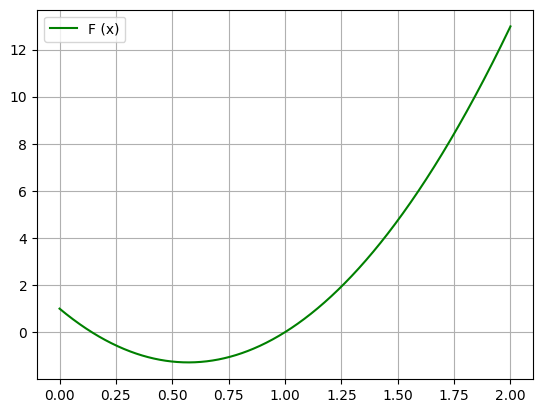
\includegraphics[width=75mm]{Figures/del1_2a_1.png} &   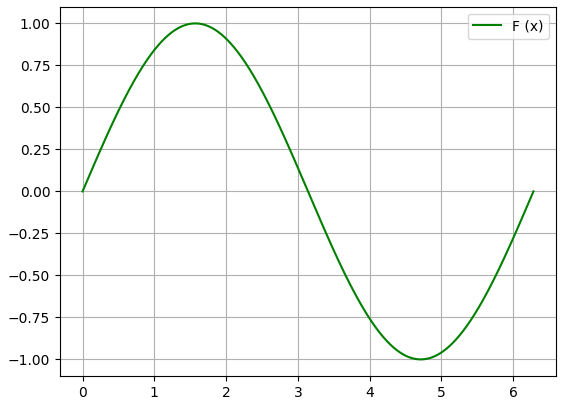
\includegraphics[width=75mm]{Figures/del1_2a_2.png} \\
            $f(x)=7x^{2}-8x+1$ & $f(x)=sin(x)$ \\[6pt]
            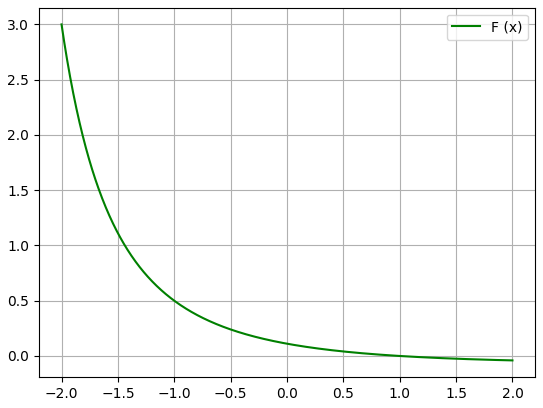
\includegraphics[width=75mm]{Figures/del1_2a_3.png} &   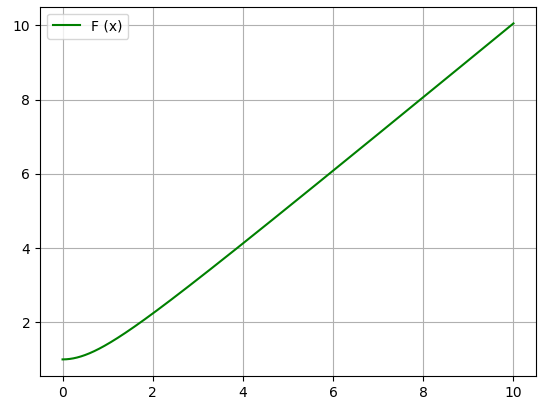
\includegraphics[width=75mm]{Figures/del1_2a_4.png} \\
            $f(x)=\frac{1-x}{(x+3)^{2}}$ & $f(x)=\sqrt{1+x^{2}}$ \\[6pt]
            \end{tabular}
        \end{figure}
        \newpage
    \subsubsection{B)} $f'(x)$
        \begin{figure}[h!]
            \begin{tabular}{cc}
            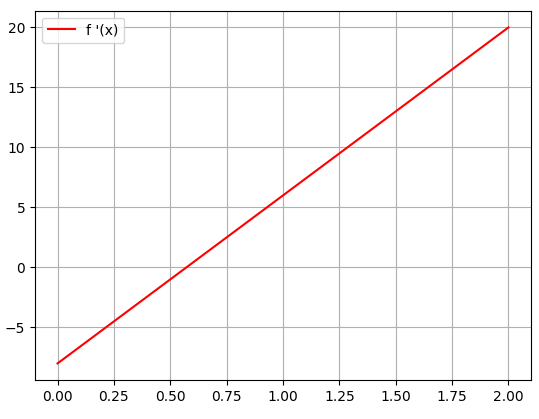
\includegraphics[width=75mm]{Figures/del1_2b_1.png} &   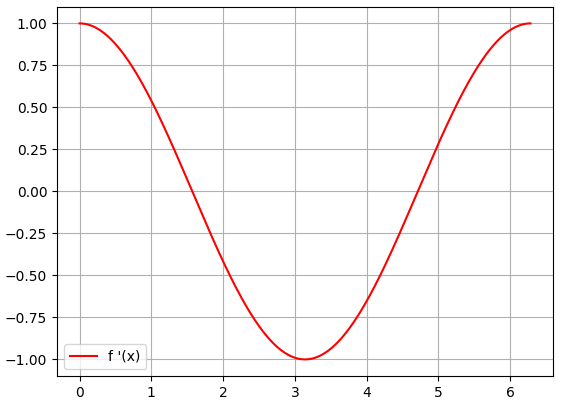
\includegraphics[width=75mm]{Figures/del1_2b_2.png} \\
            $f'(x)=14x-8$ & $f'(x)=cos(x)$ \\[6pt]
            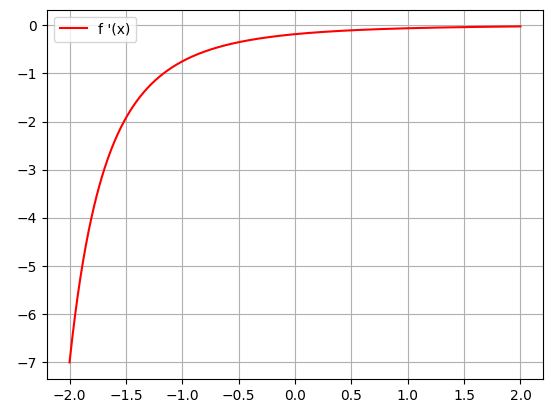
\includegraphics[width=75mm]{Figures/del1_2b_3.png} &   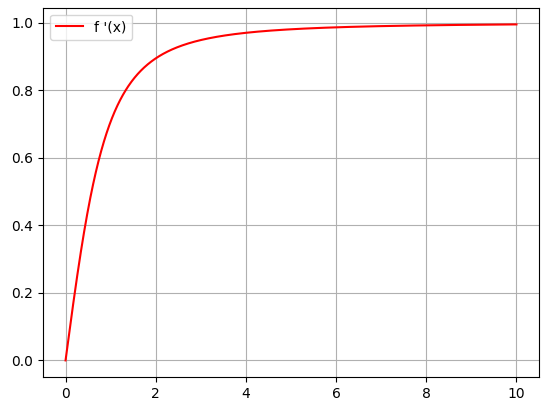
\includegraphics[width=75mm]{Figures/del1_2b_4.png} \\
            $f'(x)=\frac{x-5}{(x+3)^{3}}$ & $f'(x)=\frac{x}{\sqrt{(1+x)^{2}}}$ \\[6pt]
            \end{tabular}
        \end{figure}
        \newpage
    \subsubsection{C)} Tilnærmingen $g(x)$ med $\Delta x$ verdien fra Oppgave 1 d.
        \begin{figure}[h!]
            \begin{tabular}{cc}
            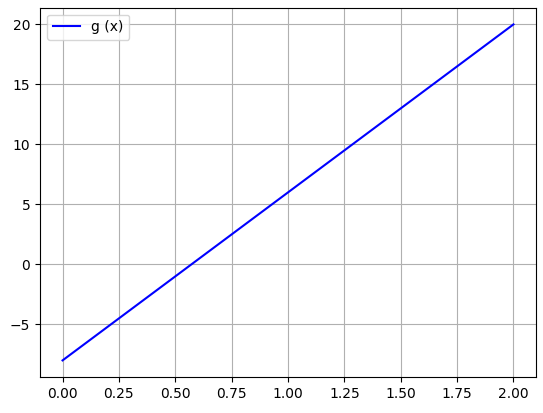
\includegraphics[width=75mm]{Figures/del1_2c_1.png} &   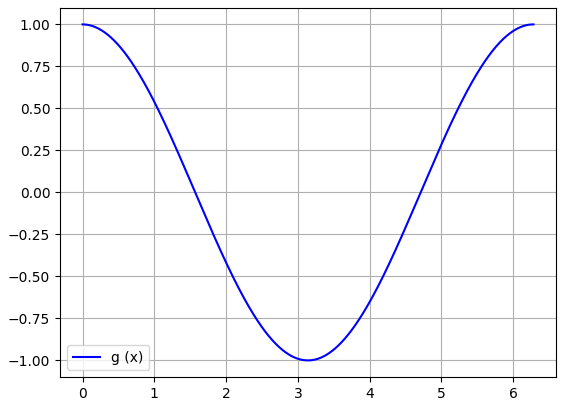
\includegraphics[width=75mm]{Figures/del1_2c_2.png} \\
            $g(x)=\frac{F(x+0.00014)-F(x)}{0.00014}$ & $g(x)=\frac{F(x+0.0028)-F(x)}{0.0028}$\\[6pt]
            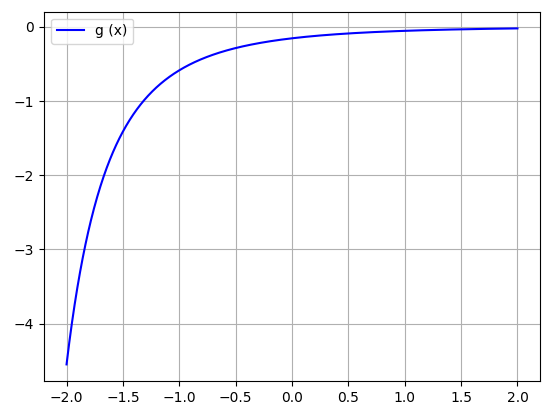
\includegraphics[width=75mm]{Figures/del1_2c_3.png} &   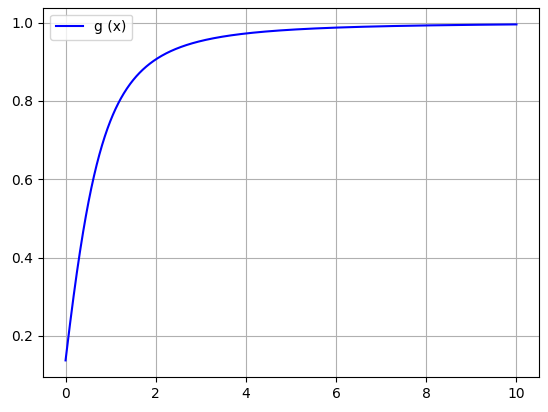
\includegraphics[width=75mm]{Figures/del1_2c_4.png} \\
            $g(x)=\frac{F(x+0.032)-F(x)}{0.032}$ & $g(x)=\frac{F(x+0.27)-F(x)}{0.27}$\\[6pt]
            \end{tabular}
        \end{figure}
        \newpage
    \subsubsection{D)} Feilen $E(x)=|f'(x) - g(x)|$\\
    MERK: I figuren for Funksjon 1 skal feilen være konstant. Variasjonen vi ser i grafen her er grunnet tallstøy/avrundingsproblemer og unøyaktigheter hos datamaskinen ved utregning av tall med mange desimaler.\\
        \begin{figure}[h!]
            \begin{tabular}{cc}
            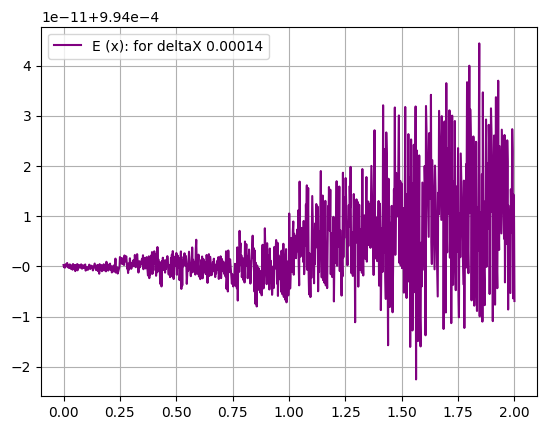
\includegraphics[width=75mm]{Figures/del1_2d_1.png} &   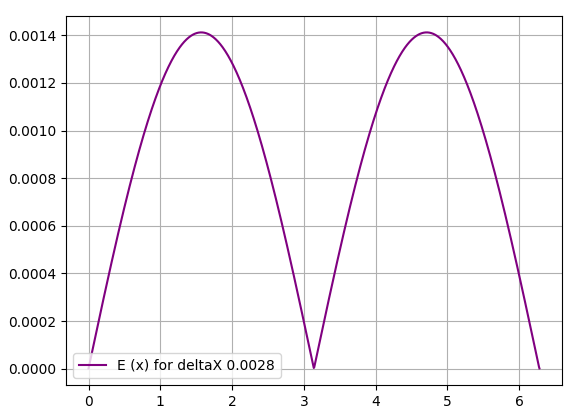
\includegraphics[width=75mm]{Figures/del1_2d_2.png} \\
            $E(x)=|f'(x) - \frac{F(x+0.00014)-F(x)}{0.00014}|$ & $E(x)=|f'(x) - \frac{F(x+0.0028)-F(x)}{0.0028}|$\\[6pt]
            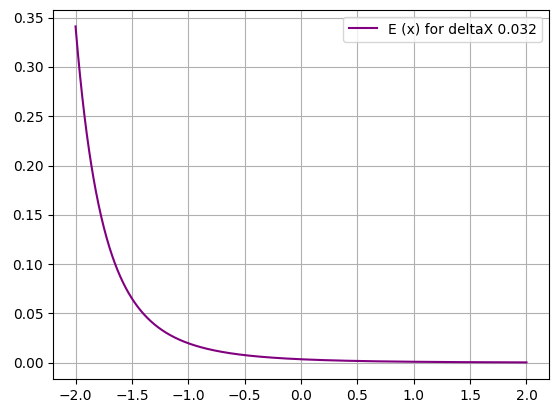
\includegraphics[width=75mm]{Figures/del1_2d_3.png} &   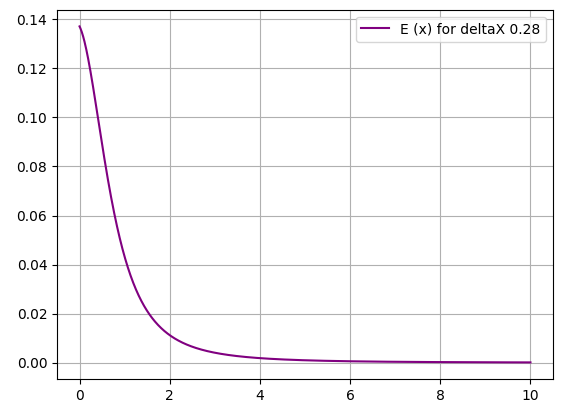
\includegraphics[width=75mm]{Figures/del1_2d_4.png} \\
            $E(x)=|f'(x) - \frac{F(x+0.032)-F(x)}{0.032}|$ & $E(x)=|f'(x) - \frac{F(x+0.27)-F(x)}{0.27}|$\\[6pt]            
            \end{tabular}
        \end{figure}
        

\section{Del 2}
\subsection{Oppgave 1}
Etter vi har satt inn $f(x)$ og $f'(x)$ ser vi at programmet konvergerer mot disse nullpunktene:
\begin{figure}[h!]
    \centering
    \begin{minipage}{0.45\textwidth}
        \centering
        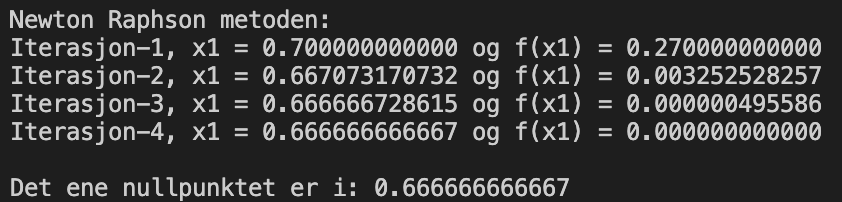
\includegraphics[width=0.9\textwidth]{Figures/del2_1_2.png}
        \caption{Startverdi: 1}
    \end{minipage}\hfill
    \begin{minipage}{0.45\textwidth}
        \centering
        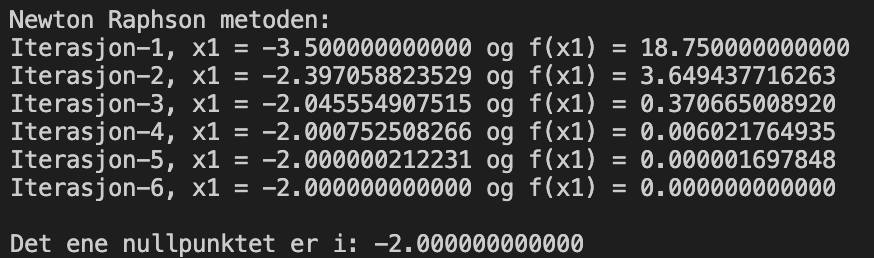
\includegraphics[width=0.9\textwidth]{Figures/del2_1_1.png}
        \caption{Startverdi: -1}
    \end{minipage}
\end{figure}
\newpage
I denne oppgaven er det bare 2 nullpunkter som du kan se på grafen av likningen under:

\begin{figure}[h!]
    \centering
    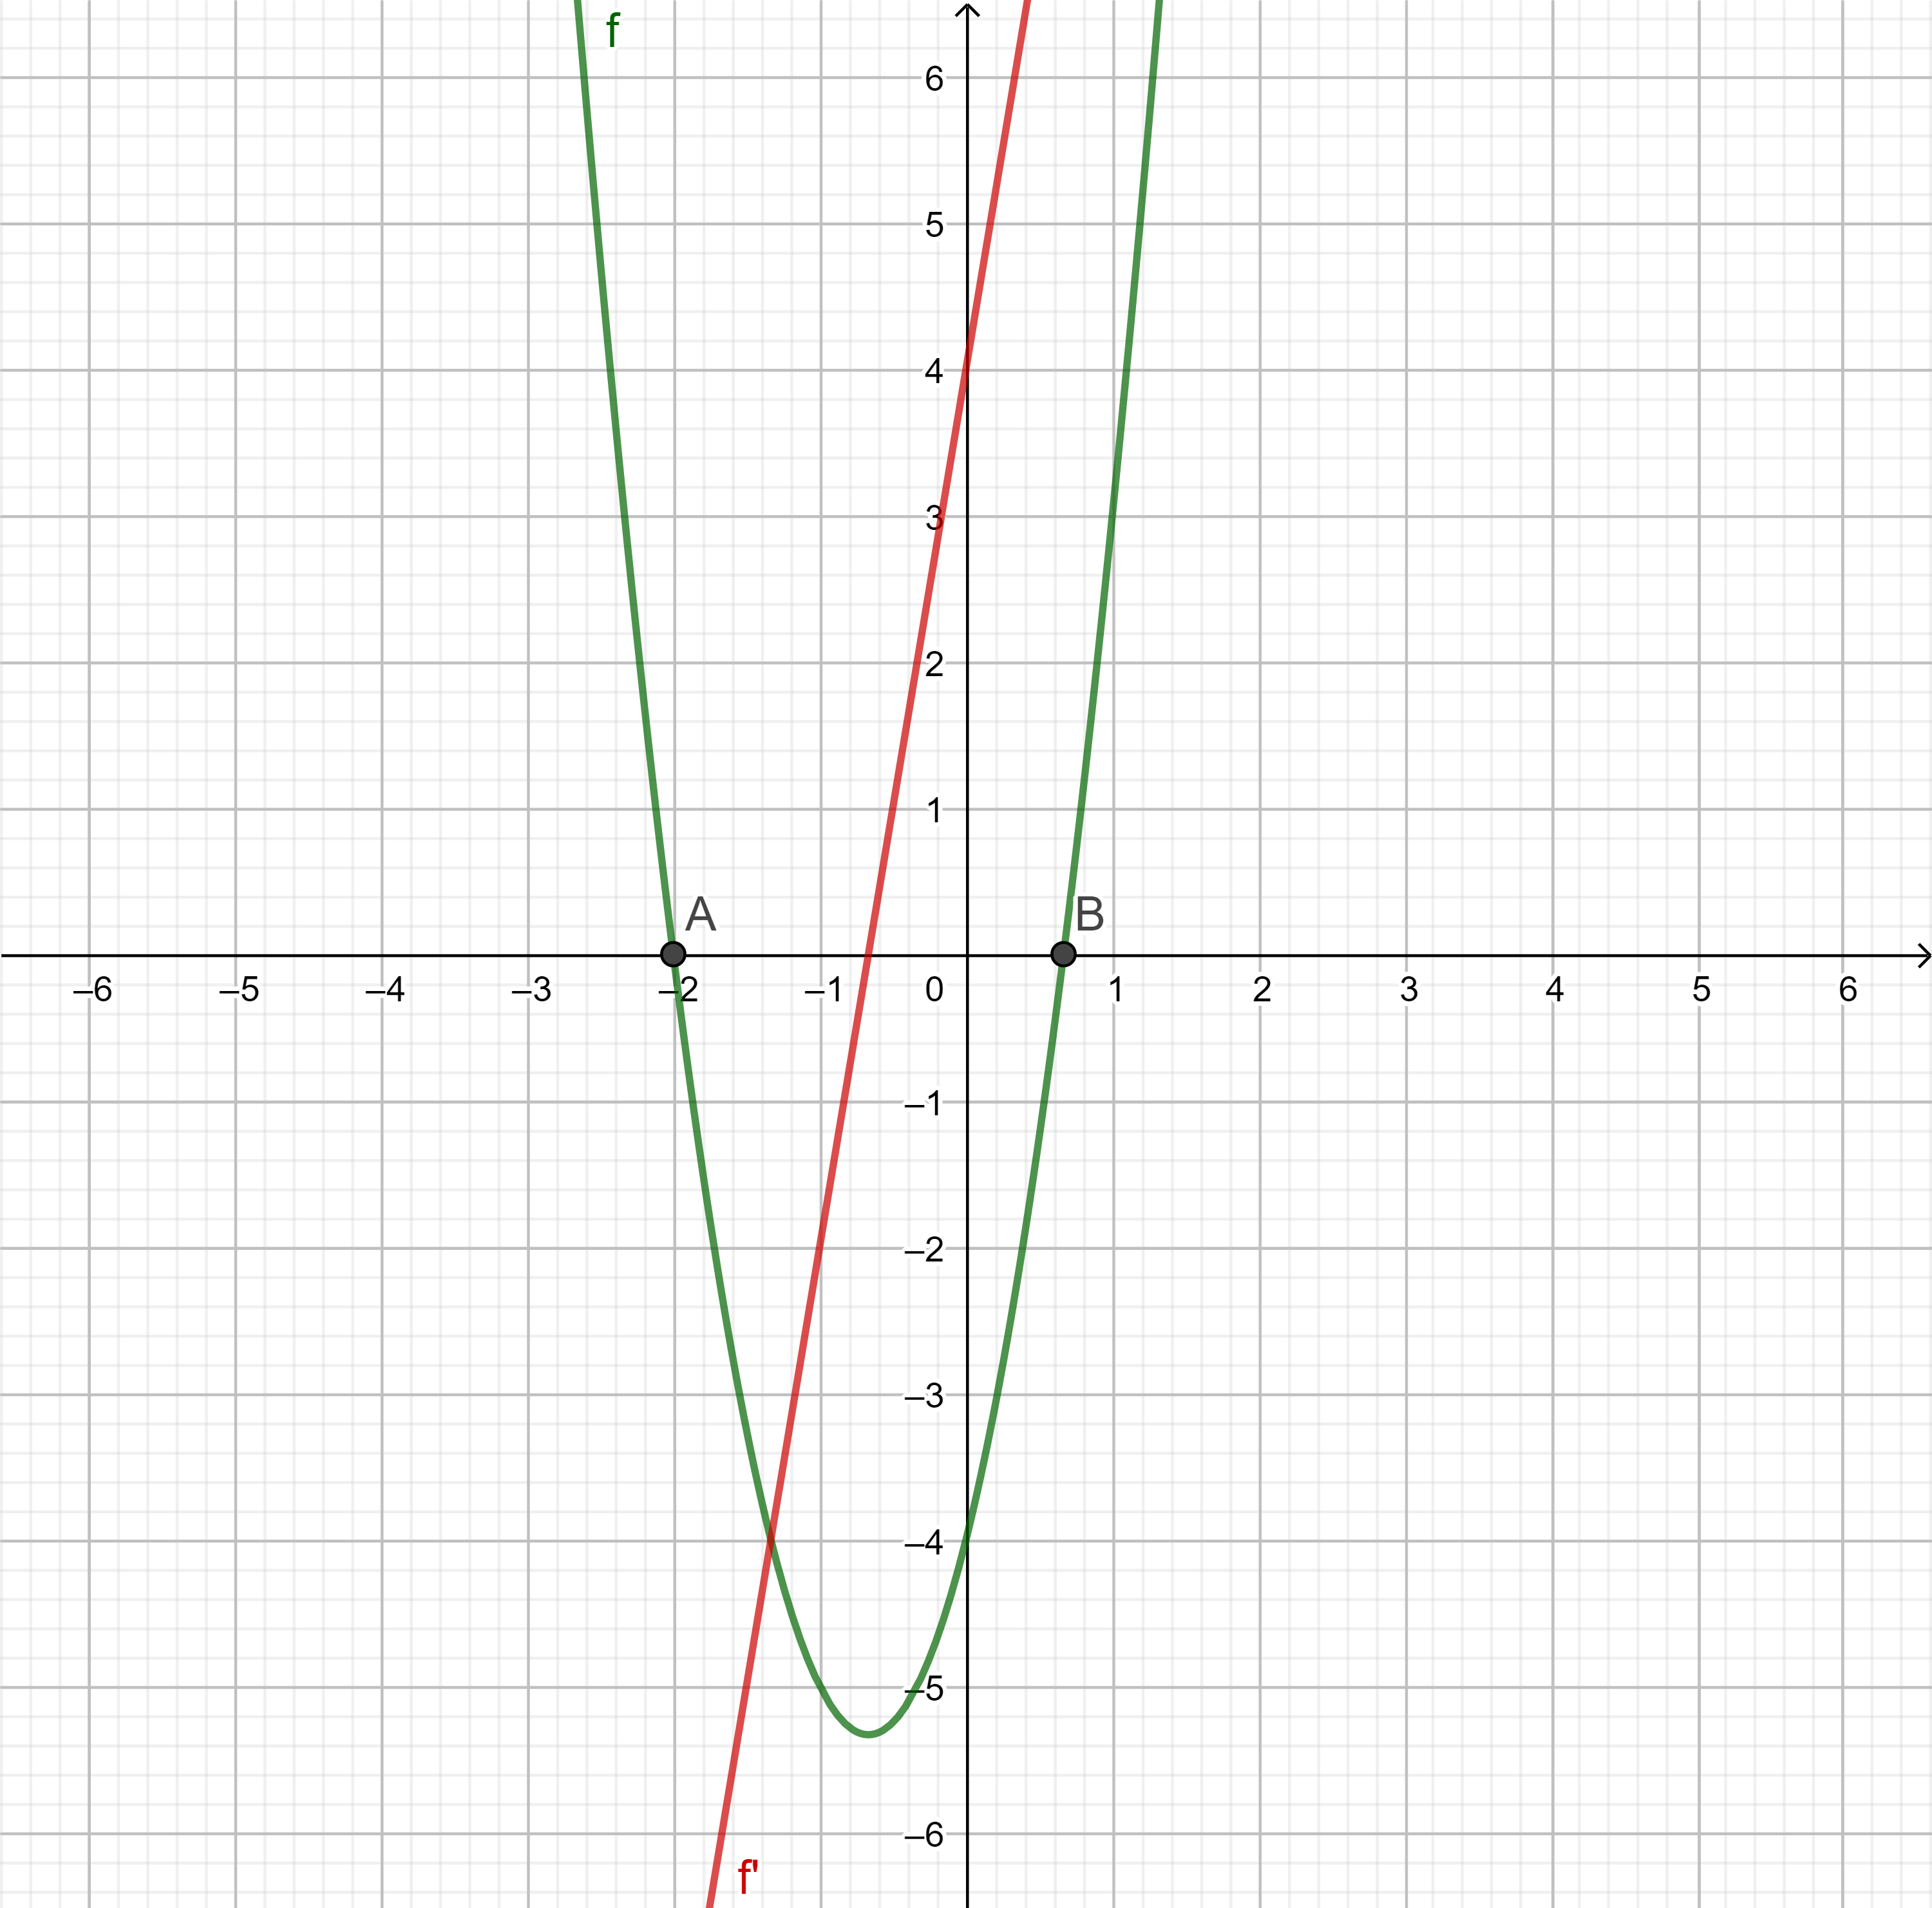
\includegraphics[width=0.40\textwidth]{Figures/Del2_1.png}
    \caption{Graf til oppgave 1, del 2}
    \label{fig:my_label}
\end{figure}

\subsection{Oppgave 2}
\subsubsection{a)}
Utledningen av likningen i denne deloppgaven:

\begin{figure}[h!]
    \centering
    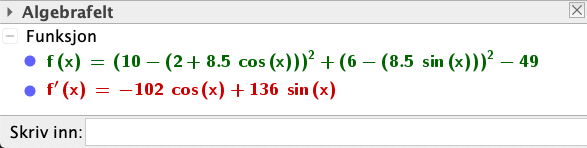
\includegraphics[width = 0.6\textwidth]{Figures/del2_2a_utledning.png}
    \caption{Utledningen gjort i GeoGebra}
    \label{fig:my_label}
\end{figure}

Etter at vi har satt inn $f(\theta_2)$ og $f'(\theta_2)$ ser vi at programmet konvergerer mot disse nullpunktene:

\begin{figure}[h!]
    \centering
    \begin{minipage}{0.45\textwidth}
        \centering
        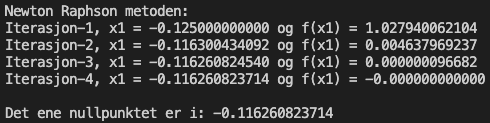
\includegraphics[width=0.9\textwidth]{Figures/del2_2a_1.png}
        \caption{Startverdi: 0}
    \end{minipage}\hfill
    \begin{minipage}{0.45\textwidth}
        \centering
        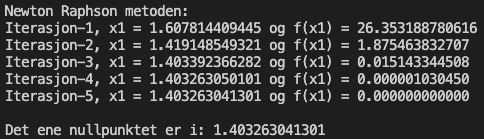
\includegraphics[width=0.9\textwidth]{Figures/del2_2a_2.png}
        \caption{Startverdi: 1}
    \end{minipage}
\end{figure}

Siden denne likningen er trigonometrisk gjelder det også for alle nullpunktene $+2k\pi$ der 'k' er større enn null og en integer. Altså for hver gang leddet i $\theta_1$ gjør en full rotasjon, kommer $\theta_2$ tilbake til samme vinkel. %Er det en bedre måte å skrive dette på?

\newpage
\subsubsection{b)}
Utledningen av likningen i denne deloppgaven:

\begin{figure}[h!]
    \centering
    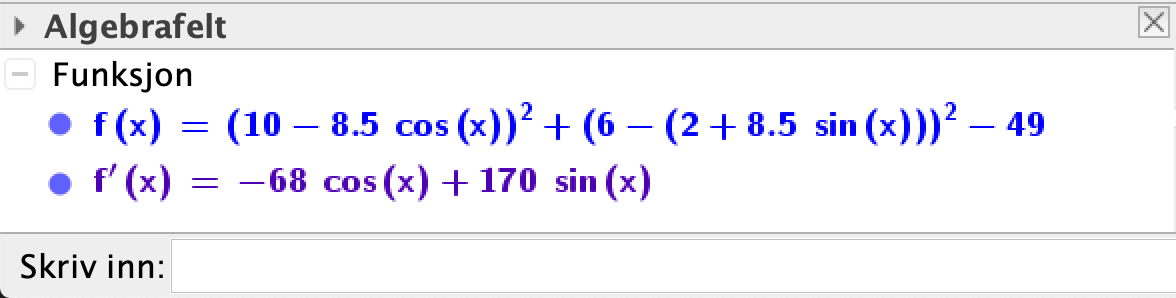
\includegraphics[width = 0.6\textwidth]{Figures/del2_2b_utledning.png}
    \caption{Utledningen gjort i GeoGebra}
    \label{fig:my_label}
\end{figure}

Etter at vi har satt inn $f(\theta_2)$ og $f'(\theta_2)$ ser vi at programmet konvergerer mot disse nullpunktene:

\begin{figure}[h!]
    \centering
    \begin{minipage}{0.45\textwidth}
        \centering
        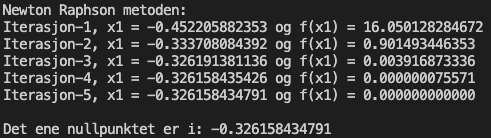
\includegraphics[width=0.9\textwidth]{Figures/del2_2b_1.png}
        \caption{Startverdi: 0}
    \end{minipage}\hfill
    \begin{minipage}{0.45\textwidth}
        \centering
        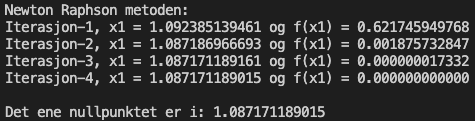
\includegraphics[width=0.9\textwidth]{Figures/del2_2b_2.png}
        \caption{Startverdi: 1}
    \end{minipage}
\end{figure}

Siden denne likningen er trigonometrisk gjelder det også for alle nullpunktene $+2k\pi$ der 'k' er større enn null og en integer. Altså for hver gang leddet i $\theta_1$ gjør en full rotasjon, kommer $\theta_2$ tilbake til samme vinkel. %Er det en bedre måte å skrive dette på?

\subsubsection{c)}
Utledningen av likningen i denne deloppgaven:

\begin{figure}[h!]
    \centering
    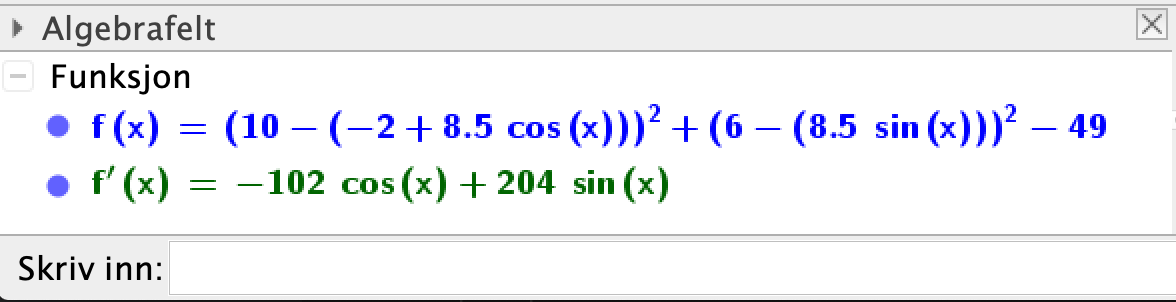
\includegraphics[width = 0.6\textwidth]{Figures/del2_2c_utledning.png}
    \caption{Utledningen gjort i GeoGebra}
    \label{fig:my_label}
\end{figure}

Etter at vi har satt inn $f(\theta_2)$ og $f'(\theta_2)$ ser vi at programmet konvergerer mot disse nullpunktene:

\begin{figure}[h!]
    \centering
    \begin{minipage}{0.45\textwidth}
        \centering
        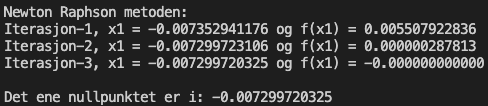
\includegraphics[width=0.95\textwidth]{Figures/del2_2c_1.png}
        \caption{Startverdi: 0}
    \end{minipage}\hfill
    \begin{minipage}{0.45\textwidth}
        \centering
        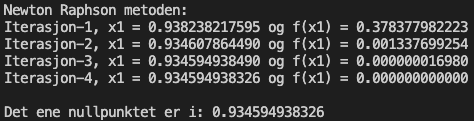
\includegraphics[width=0.9\textwidth]{Figures/del2_2c_2.png}
        \caption{Startverdi: 1}
    \end{minipage}
\end{figure}

Siden denne likningen er trigonometrisk gjelder det også for alle nullpunktene $+2k\pi$ der 'k' er større enn null og en integer. Altså for hver gang leddet i $\theta_1$ gjør en full rotasjon, kommer $\theta_2$ tilbake til samme vinkel. %Er det en bedre måte å skrive dette på? 
 
\chapter{Diskusjon} \\
\textbullet \textbf{Sammenhengen mellom \pmb{$f(x)$} og \pmb{$f'(x)$}. F.eks. hvordan \pmb{$f'(x)$} varierer i forhold til \pmb{$f(x)$}.}\\
\\
$f'(x)$ viser stigningen i $f(x)$ og hvordan den endrer seg, med tanke på x. Vi bruker det hvis vi vil komme frem til hvor mye en funksjon stiger i ett visst punkt. \\
\\
\textbullet \textbf{Hvordan valg av \pmb{$\Delta x$} påvirker nøyaktigheten av tilnærmingene. F.eks. hvor liten kan vi velge \pmb{$\Delta x$} ?\\}
\\
Valget av  $\Delta x$ påvirker nøyaktigheten av tilnærmingene vi gjør. Fordi jo lavere $\Delta x$ vi velger, jo nærmere den faktiske x-verdien er vi. Men når vi velger $\Delta x$ kommer vi til ett punkt hvor det ikke gir mening og velge en lavere verdi. Hvis vi bare vil vise 2 desimaler i svaret gir det ikke mening og velge en $\Delta x > 0.01$.\\
\\
\textbullet \textbf{Hvordan feilen \pmb{$E(x)$} varierer som en funksjon av \pmb{$x$}.\\}
\\
Feilen $E(x)$ vil bli større jo større verdi for x vi putter inn. Ettersom tilnærmingenene og nøyaktigheten vil bli mindre desto mindre verdi for x man velger for $\Delta x$. Hvis funksjonen $f(x)$ ikke er lineær, vil man se at desto lengre vekk man kommer fra det punktet man deriverer i desto større blir feilen.\\ I flere av funksjonene ser vi også en sammenheng mellom $E(x)$ og den annenderiverte $f''(x)$ til funksjonen. De tydeligste eksemplene på dette er Funksjon 1, hvor den annenderiverte er en konstant, og funksjon 2, hvor E, når amplituden blåses opp tilstrekkelig, er en ganske tro gjenskapning av |-sin(x)|, dvs absoluttverdien til den annenderiverte av sin(x).
\\
\textbullet \textbf{Begrensninger ved numeriske tilnærminger av den deriverte.\\}
\\
Begrensningene med den numeriske tilnærmingen av den deriverte er det at vi ikke får en nøyaktig derivert. Altså den vil alltid ha en viss feilmargin. Eneste måten å unngå dette er ved å bruke den eksakte deriverte. \\
\\
\textbullet \textbf{Utforsk den fysiske betydningen av de to løsningene i hvert tilfelle.\\}
\\
Når vi finner nullpunktene til $\theta_2$ får vi 2 verdier, her er den ene verdien for når armen til derricken er bøyd opp, og den andre verdien er når d en er bøyd ned, og den vil aldri bytte mellom disse tilstandene. 
\\
\\
\newpage
\textbullet \textbf{Finn sammenhengen mellom initialverdien brukt i løsningsmetoden, og hvilken av de to løsningene metoden konvergerer mot.\\}
\\
Sammenhengen mellom initialverdien og nullpunktet den konvergerer mot er at hvis du velger initialverdi hvor stigningstallet til funksjonen er negativt konvergerer du mot det de nullpunktet der derricken er bøyd nedover. Velger du initialverdi hvor stigningstallet til funksjonen er positivt konvergerer du mot de nullpunktene hvor derricken er bøyd oppover. Dette gjelder derimot ikke hvis vi velger verdier nærme topp- og bunnpunkter, fordi da er stigningstallet 0.
\chapter{Konklusjon}

I dette prosjektet har vi gått igjennom og lært om de matematiske metodene Numerisk tilnærming av den deriverte og Newton-Raphson metoden. Prosjektet har hatt fokus på å utfordre oss innenfor disse områdene og vi har lært ulike konsepter og metoder vi kan bruke til å løse slike problemer på. Vi har blitt bedre kjent med reglene for disse regnemetodene og generelt fått en god forståelse for de forskjellige metodene vi bruker.
\\
\\ 
Etter å ha jobbert med det prosjektet, lærte vi kjente derivasjon regler og bruk av dem for å komme frem til løsningen. I tillegg har vi lært og brukt Limit til å finne en tilnærming til den deriverte av en gitt funksjon når differansen på x-verdiene går mot null. 
\\
\\ 
Gjennom Newton-Raphson metoden lærte vi hvordan vi kunne bruke en funksjon og dens deriverte til å finne en god tilnærming til nullpunktene til funksjonen, så lenge gjennomsnittsveksten ikke er lik null. Andre ting vi oppdaget igjennom oppgaven var at Newton-Raphson metoden ikke alltid fungerer. Det er visse punkter den ikke fungerer i, som for eksempel når $f'(x) = 0$. \\
\\
Alt i alt har dette prosjektet vært en bra lære opplevelse for vår gruppe, og vi har fått stort utbytte av det. Det har vært generelt gode og overkommelige oppgaver som fortsatt ga oss en viss utfordring. 


\printbibliography[
heading=bibintoc,
title={Bibliografi}
]

\appendix

\chapter{Kode}
Kodekommentarer kommer ikke frem like tydelig som ønskelig her, den wrappes også videre over til ny side ved flere steder, noe som ødelegger kontinuitet i lesningen. Dette er beklagelig.\\
Ved ønske om nærmere gransking av koden i mer kode-vennlig medium, se Github.\cite{github}
\section{Del 1}\label{app:d1o1&2}
Koden for Oppgave 1D og Oppgave 2 er gjort i samme fil, separert for hver av de fire funksjonene.
\subsection{Funksjon 1}
\label{app:func1}
\begin{lstlisting}
import numpy as np
import matplotlib.pyplot as plt 

x0 = 1
min = 0
max = 2

def f(x):
    return (14*x) - 8

def g(dx,x=x0):
    return np.longdouble((F(x+dx)-F(x))/dx)

def G(x): #To funksjoner for tilnærmingen g fordi dette gjør det enklere å tegne grafen separert fra f'
    return np.longdouble((F(x+0.00014)-F(x))/0.00014) #DeltaX hardkodet inn etter funn i Del1:Oppgave1D

def F(x):
    return 7*x**2 -8*x +1


for x in np.arange(0,0.001,0.000001): #Loop for å finne største gyldige DeltaX for E<=0.001. Loop grenser og stepsize funnet ved prøv&feil
    Ex = abs(f(x0)-g(dx=x))
    if(Ex<=0.001):
        valid=x
        #print("F:{0}, G:{1}, f:{2}, E:{3}, x:{4}".format(F(x0+x),g(x),f(x0),Ex,x))#Fjern '#' tegnet foran denne linjen for å kjøre koden med printing av E og deltaX
    elif(Ex>0.001):
        break

i=0
E = [0]*1000
for x in np.linspace(min,max,1000): #Loop for å beregne variasjon i E over et gitt intervall min -> max
    E[i] = abs(f(x)-g(x=x,dx=valid))
    i+=1


fig = plt.gcf()
fig.canvas.set_window_title('Funksjon 1: 7x² - 8x + 1')
x=np.linspace(min,max,1000)
y=F(x)
yd=f(x)
yg=G(x)
ye=E
plt.grid(True)
plt.plot(x,yd,'r-', label='f \'(x)')
plt.plot(x,y,'g-',label="F (x)")
plt.plot(x,yg,'b-',label="g (x)")
plt.plot(x,ye,color='purple',label='E (x): for deltaX %.5f'%(valid))
plt.legend()    
plt.show()

\end{lstlisting}
\subsection{Funksjon 2}
\label{app:func2}
\begin{lstlisting}
import numpy as np
import matplotlib.pyplot as plt 

x0 = np.pi/4
min = 0
max = 2*np.pi

def f(x):
    return np.cos(x)

def g(dx,x=x0):
    return np.longdouble((F(x+dx)-F(x))/dx)

def G(x):  #To funksjoner for tilnærmingen g fordi dette gjør det enklere å tegne grafen separert fra f'
    return np.longdouble((F(x+0.002825)-F(x))/0.002825)#DeltaX hardkodet inn etter funn i Del1:Oppgave1D

def F(x):
    return np.sin(x)

for x in np.arange(0,0.01,0.000001):#Loop for å finne største gyldige DeltaX for E<=0.001. Loop grenser og stepsize funnet ved prøv&feil
    Ex = abs(f(x0)-g(x))
    if(Ex<=0.001):
        valid=x
        #print("F:{0}, G:{1}, f:{2}, E:{3}, x:{4}".format(F(x0+x),g(x),f(x0),Ex,x)) #Fjern '#' tegnet foran denne linjen for å kjøre koden med printing av E og deltaX
    elif(Ex>0.001):
        break

i=0
E = [0]*1000
for x in np.linspace(min,max,1000): #Loop for å beregne variasjon i E over et gitt intervall min -> max
    E[i] = np.longdouble(abs(f(x)-g(x=x,dx=valid)))
    i+=1

fig = plt.gcf()
fig.canvas.set_window_title('Funksjon 2: sin(x)')
x=np.array(np.linspace(min,max,1000))
y=F(x)
yd=f(x)
yg=G(x)
ye=E
plt.grid(True)
plt.plot(x,yd,'r-', label='f \'(x)')
plt.plot(x,y,'g-',label="F (x)")
plt.plot(x,yg,'b-',label="g (x)")
plt.plot(x,ye,color='purple',label='E (x) for deltaX %.4f'%(valid))
plt.legend()    
plt.show()
\end{lstlisting}
\subsection{Funksjon 3}
\label{app:func3}
\begin{lstlisting}
import numpy as np
import matplotlib.pyplot as plt 

x0 = 1
min = -2
max = 2

def f(x):
    return (x-5)/(x+3)**3

def g(dx,x=x0):
    return np.longdouble((F(x+dx)-F(x))/dx)

def G(x):  #To funksjoner for tilnærmingen g fordi dette gjør det enklere å tegne grafen separert fra f'
    return np.longdouble((F(x+0.32389)-F(x))/0.32389)#DeltaX hardkodet inn etter funn i Del1:Oppgave1D

def F(x):
    return (1-x)/((x+3)**2)


for x in np.arange(0.032,0.1,0.000001):#Loop for å finne største gyldige DeltaX for E<=0.001. Loop grenser og stepsize funnet ved prøv&feil
    Ex = abs(f(x0)-g(x))
    if(Ex<=0.001):
        valid=x
        #print("F:{0}, G:{1}, f:{2}, E:{3}, x:{4}".format(F(x0+x),g(x),f(x0),Ex,x))#Fjern '#' tegnet foran denne linjen for å kjøre koden med printing av E og deltaX
    elif(Ex>0.001):
        break

i=0
E = [0]*1000
for x in np.linspace(min,max,1000): #Loop for å beregne variasjon i E over et gitt intervall min -> max
    E[i] = np.longdouble(abs(f(x)-g(x=x,dx=valid)))
    i+=1

fig = plt.gcf()
fig.canvas.set_window_title('Funksjon 3: (1-x)/(x+3)²')
x=np.linspace(min,max,1000)
y=F(x)
yd=f(x)
yg=G(x)
ye=E
plt.grid(True)
plt.plot(x,yd,'r-', label='f \'(x)')
plt.plot(x,y,'g-',label="F (x)")
plt.plot(x,yg,'b-',label="g (x)")
plt.plot(x,ye,color='purple',label='E (x) for deltaX %.3f'%(valid))
plt.legend()    
plt.show()
\end{lstlisting}
\subsection{Funksjon 4}
\label{app:func4}
\begin{lstlisting}
import numpy as np
import matplotlib.pyplot as plt 

x0 = 5
min = 0
max = 10

def f(x):
    return x/np.sqrt(1+x**2)

def g(dx,x=x0):
    return np.longdouble((F(x+dx)-F(x))/dx)

def G(x):  #To funksjoner for tilnærmingen g fordi dette gjør det enklere å tegne grafen separert fra f'
    return np.longdouble((F(x+0.28)-F(x))/0.28)#DeltaX hardkodet inn etter funn i Del1:Oppgave1D

def F(x):
    return np.sqrt(1+x**2)


for x in np.arange(0.279,max-x0,0.000001):#Loop for å finne største gyldige DeltaX for E<=0.001. Loop grenser og stepsize funnet ved prøv&feil
    Ex = abs(f(x0)-g(x))
    if(Ex<=0.001):
        valid=x
        #print("F:{0}, G:{1}, f:{2}, E:{3}, x:{4}".format(F(x0+x),g(x),f(x0),Ex,x))#Fjern '#' tegnet foran denne linjen for å kjøre koden med printing av E og deltaX
    elif(Ex>0.001):
        break

i=0
E = [0]*1000
for x in np.linspace(min,max,1000): #Loop for å beregne variasjon i E over et gitt intervall min -> max
    E[i] = np.longdouble(abs(f(x)-g(x=x,dx=valid)))
    i+=1


fig = plt.gcf()
fig.canvas.set_window_title('Funksjon 4: sqrt(1+x²)')
x=np.linspace(min,max,1000)
y=F(x)
yd=f(x)
yg=G(x)
ye=E
plt.grid(True)
plt.plot(x,yd,'r-', label='f \'(x)')
plt.plot(x,y,'g-',label="F (x)")
plt.plot(x,yg,'b-',label="g (x)")
plt.plot(x,ye,color='purple',label='E (x) for deltaX %.2f'%(valid))
plt.legend()    
plt.show()
\end{lstlisting}

\section{Del 2}
\subsection{Oppgave 1}
\begin{lstlisting}
'''
Denne koden tregner 1 input fra brukeren. Den trenger en startverdi på hvor
man tror det ene nullpunktet er. Hvis startverdien er nærme nok til at det kommer innenfor feilmarginen
før antall iterasjoner er nådd vil den si hvor nullpunktet er.

Hvis man ikke skulle komme frem til nullpunktet innen antallet iterasjoner jeg har lagt inn i koden
kan man i praksis øke dette tallet, men man har generelt valgt en dårlig start verdi om den skulle trenge
flere itersajoner...
'''

def f(x):
    return 3*x**2 + 4*x - 4

def g(x):
    return 6*x + 4

def newtonRaphson(x0,e,I):
    print('\nNewton Raphson metoden:')
    step = 1
    flag = 1
    condition = True

    while condition:
        if(g(x0) == 0.0): # Hvis startverdien vi skriver inn gjør den deriverte lik 0 stopper koden, kan ikke dele på 0
            print("kan ikke dele på 0")
            break
        
        x1 = x0 - f(x0)/g(x0)
        print('Iterasjon-%d, x1 = %0.12f og f(x1) = %0.12f' % (step, x1, f(x1)))
        x0 = x1
        step = step + 1

        if step > I:
            flag = 0
            break

        condition = abs(f(x1)) > e

    if flag == 1:
        print('\nDet ene nullpunktet er i: %0.12f' % x1)
    else:
        print("\nIkke konvergent.")

x0 = input("Startverdi: ") #Startverdi
e = 10**(-12) #max tillatte feilen
I = 100 #Max antall iterasjoner

x0 = float(x0)
e = float(e)
I = int(I) 

newtonRaphson(x0,e,I)
\end{lstlisting}

\subsection{Oppgave 2a}
\begin{lstlisting}
'''
Denne koden trenger 1 input fra brukeren. Den trenger en startverdi på hvor
man tror det ene nullpunktet er som da er . Hvis startverdien er nærme nok til at det kommer innenfor feilmarginen
før antall iterasjoner er nådd vil den si hvor nullpunktet er.

Hvis man ikke skulle komme frem til nullpunktet innen antallet iterasjoner jeg har lagt inn i koden
kan man i praksis øke dette tallet, men man har generelt valgt en dårlig start verdi om den skulle trenge
flere itersajoner...

Gode startverider er typisk verdier som er relativt nærme nullpunkter til grafen. 
For denne grafen er gode startverdier f.eks.: "0" og "1"

Siden denne grafen er en trigonometrisk funksjon fortsetter den ut i uendelighet, derfor kan vi også plusse på 2*pi*k
der k er en integer, fordi det er nullpunkter i alle disse verdiene ut i uendeligheten.
'''

import math

x0 = input("Startverdi: ") #Startverdi
e = 10**(-12) #Max tillatte feilen
I = 100 #Max antall iterasjonerr

x0 = float(x0)
e = float(e)
I = int(I)

x = x0
cos = math.cos
sin = math.sin

def f(x):
    return (10 - (2 + 8.5*cos(x)))**2 + (6 - (8.5*sin(x)))**2 - 49

def g(x):
    return -102*cos(x) + 136*sin(x)

def newtonRaphson(x0,e,I):
    print('\nNewton Raphson metoden:')
    step = 1
    flag = 1
    condition = True

    while condition:
        if(g(x0) == 0.0): # Hvis startverdien vi skriver inn gjør den deriverte lik 0 stopper koden, kan ikke dele på 0
            print("kan ikke dele på 0")
            break
        
        x1 = x0 - f(x0)/g(x0)
        print('Iterasjon-%d, x1 = %0.12f og f(x1) = %0.12f' % (step, x1, f(x1)))
        x0 = x1
        step= step + 1

        if step > I:
            flag = 0
            break

        condition = abs(f(x1)) > e

    if flag == 1:
        print('\nDet ene nullpunktet er i: %0.12f' % x1)
    else:
        print("\nIkke konvergent.")

newtonRaphson(x0,e,I)
\end{lstlisting}

\subsection{Oppgave 2b}
\begin{lstlisting}
'''
Denne koden tregner 1 input fra brukeren. Den trenger en startverdi på hvor
man tror det ene nullpunktet er. Hvis startverdien er nærme nok til at det kommer innenfor feilmarginen
før antall iterasjoner er nådd vil den si hvor nullpunktet er.

Hvis man ikke skulle komme frem til nullpunktet innen antallet iterasjoner jeg har lagt inn i koden
kan man i praksis øke dette tallet, men man har generelt valgt en dårlig start verdi om den skulle trenge
flere itersajoner...

Gode startverider er typisk verdier som er relativt nærme nullpunkter til grafen. 
For denne grafen er gode startverdier f.eks.: "0" og "1"

Siden denne grafen er en trigonometrisk funksjon fortsetter den ut i uendelighet, derfor kan vi også plusse på 2*pi*k
der k er en integer, fordi det er nullpunkter i alle disse verdiene ut i uendeligheten.
'''

import math

x0 = input("Startverdi: ") #Startverdi
e = 10**(-12) #Max tillatte feilen
I = 100 #Max antall iterasjoner

x0 = float(x0)
e = float(e)
I = int(I)

x = x0
cos = math.cos
sin = math.sin

def f(x):
    return (10 - (8.5*cos(x)))**2 + (6 - (2 + 8.5*sin(x)))**2 - 49

def g(x):
    return -68*cos(x) + 170*sin(x)

def newtonRaphson(x0,e,I):
    print('\nNewton Raphson metoden:')
    step = 1
    flag = 1
    condition = True

    while condition:
        if(g(x0) == 0.0): # Hvis startverdien vi skriver inn gjør den deriverte lik 0 stopper koden, kan ikke dele på 0
            print("kan ikke dele på 0")
            break
        
        x1 = x0 - f(x0)/g(x0)
        print('Iterasjon-%d, x1 = %0.12f og f(x1) = %0.12f' % (step, x1, f(x1)))
        x0 = x1
        step = step + 1

        if step > I:
            flag = 0
            break

        condition = abs(f(x1)) > e

    if flag == 1:
        print('\nDet ene nullpunktet er i: %0.12f' % x1)
    else:
        print("\nIkke konvergent.")

newtonRaphson(x0,e,I)
\end{lstlisting}

\subsection{Oppgave 2c}
\begin{lstlisting}
'''
Denne koden tregner 1 input fra brukeren. Den trenger en startverdi på hvor
man tror det ene nullpunktet er. Hvis startverdien er nærme nok til at det kommer innenfor feilmarginen
før antall iterasjoner er nådd vil den si hvor nullpunktet er.

Hvis man ikke skulle komme frem til nullpunktet innen antallet iterasjoner jeg har lagt inn i koden
kan man i praksis øke dette tallet, men man har generelt valgt en dårlig start verdi om den skulle trenge
flere itersajoner...

Gode startverider er typisk verdier som er relativt nærme nullpunkter til grafen. 
For denne grafen er gode startverdier f.eks.: "0" og "1"

Siden denne grafen er en trigonometrisk funksjon fortsetter den ut i uendelighet, derfor kan vi også plusse på 2*pi*k
der k er en integer, fordi det er nullpunkter i alle disse verdiene ut i uendeligheten.
'''

import math

x0 = input("Startverdi: ") #Startverdi
e = 10**(-12) #Max tillatte feilen
I = 100 #Max antall iterasjoner

x0 = float(x0)
e = float(e)
I = int(I)

x = x0
cos = math.cos
sin = math.sin

def f(x):
    return (10 - (-2 + 8.5*cos(x)))**2 + (6 - (8.5*sin(x)))**2 - 49

def g(x):
    return -102*cos(x) + 204*sin(x)

def newtonRaphson(x0,e,I):
    print('\nNewton Raphson metoden:')
    step = 1
    flag = 1
    condition = True

    while condition:
        if(g(x0) == 0.0): # Hvis startverdien vi skriver inn gjør den deriverte lik 0 stopper koden, kan ikke dele på 0
            print("kan ikke dele på 0")
            break
        
        x1 = x0 - f(x0)/g(x0)
        print('Iterasjon-%d, x1 = %0.12f og f(x1) = %0.12f' % (step, x1, f(x1)))
        x0 = x1
        step = step + 1

        if step > I:
            flag = 0
            break

        condition = abs(f(x1)) > e

    if flag == 1:
        print('\nDet ene nullpunktet er i: %0.12f' % x1)
    else:
        print("\nIkke konvergent.")

newtonRaphson(x0,e,I)
\end{lstlisting}



\end{document}

